\section{Experiments}
\label{sec:experiments}

We will now return to the original question of the paper: Is planning
technology ready for applications in natural language generation? We
will tackle this question by evaluating the performance of several
planners on the NLG planning domains from the previous section.

We start with two experiments in the CRISP domain. First, we present a
scenario which focuses on the generation of referring expressions with
a tiny grammar (Section~\ref{sec:exper-1:-sent}); then we look at a
setting in which CRISP is used for surface realization with the XTAG
Grammar \citep{xtag01:_tr}, a large-scale TAG grammar of English
(Section~\ref{sec:exper-2:-sent-xtag}).

We then go through a series of experiments in the GIVE domain. We
start with a domain that is essentially Gridworld
(Section~\ref{sec:exper-2:-minim}), and then add positions that are
either not needed (Section~\ref{sec:experiment-3:-give}) or even
inaccessible (Section~\ref{sec:experiment-4:-give}).


\subsection{Experiment 1: Sentence generation (referring expressions)}
\label{sec:exper-1:-sent}

In the first experiment, we construct a series of sentence generation
problems which require the planner to compute a plan representing the
sentence ``Mary likes the Adj$_1$ \ldots Adj$_n$ rabbit.''  Each problem
instance assumes a certain number $m$ of rabbits that were distinguished by
$n \leq m$ different properties, such that all $n$ properties are required
to distinguish the target referent from all other rabbits.  The $n$
properties are realized as $n$ different adjectives, in any order.  This
setup allows us to control the plan length (a plan with $n$ properties will
have length $n+4$) and the universe size (the universe will contain $m+1$
individuals in addition to the differently-typed individuals used to encode
the grammar).

\begin{figure}
  \centering
  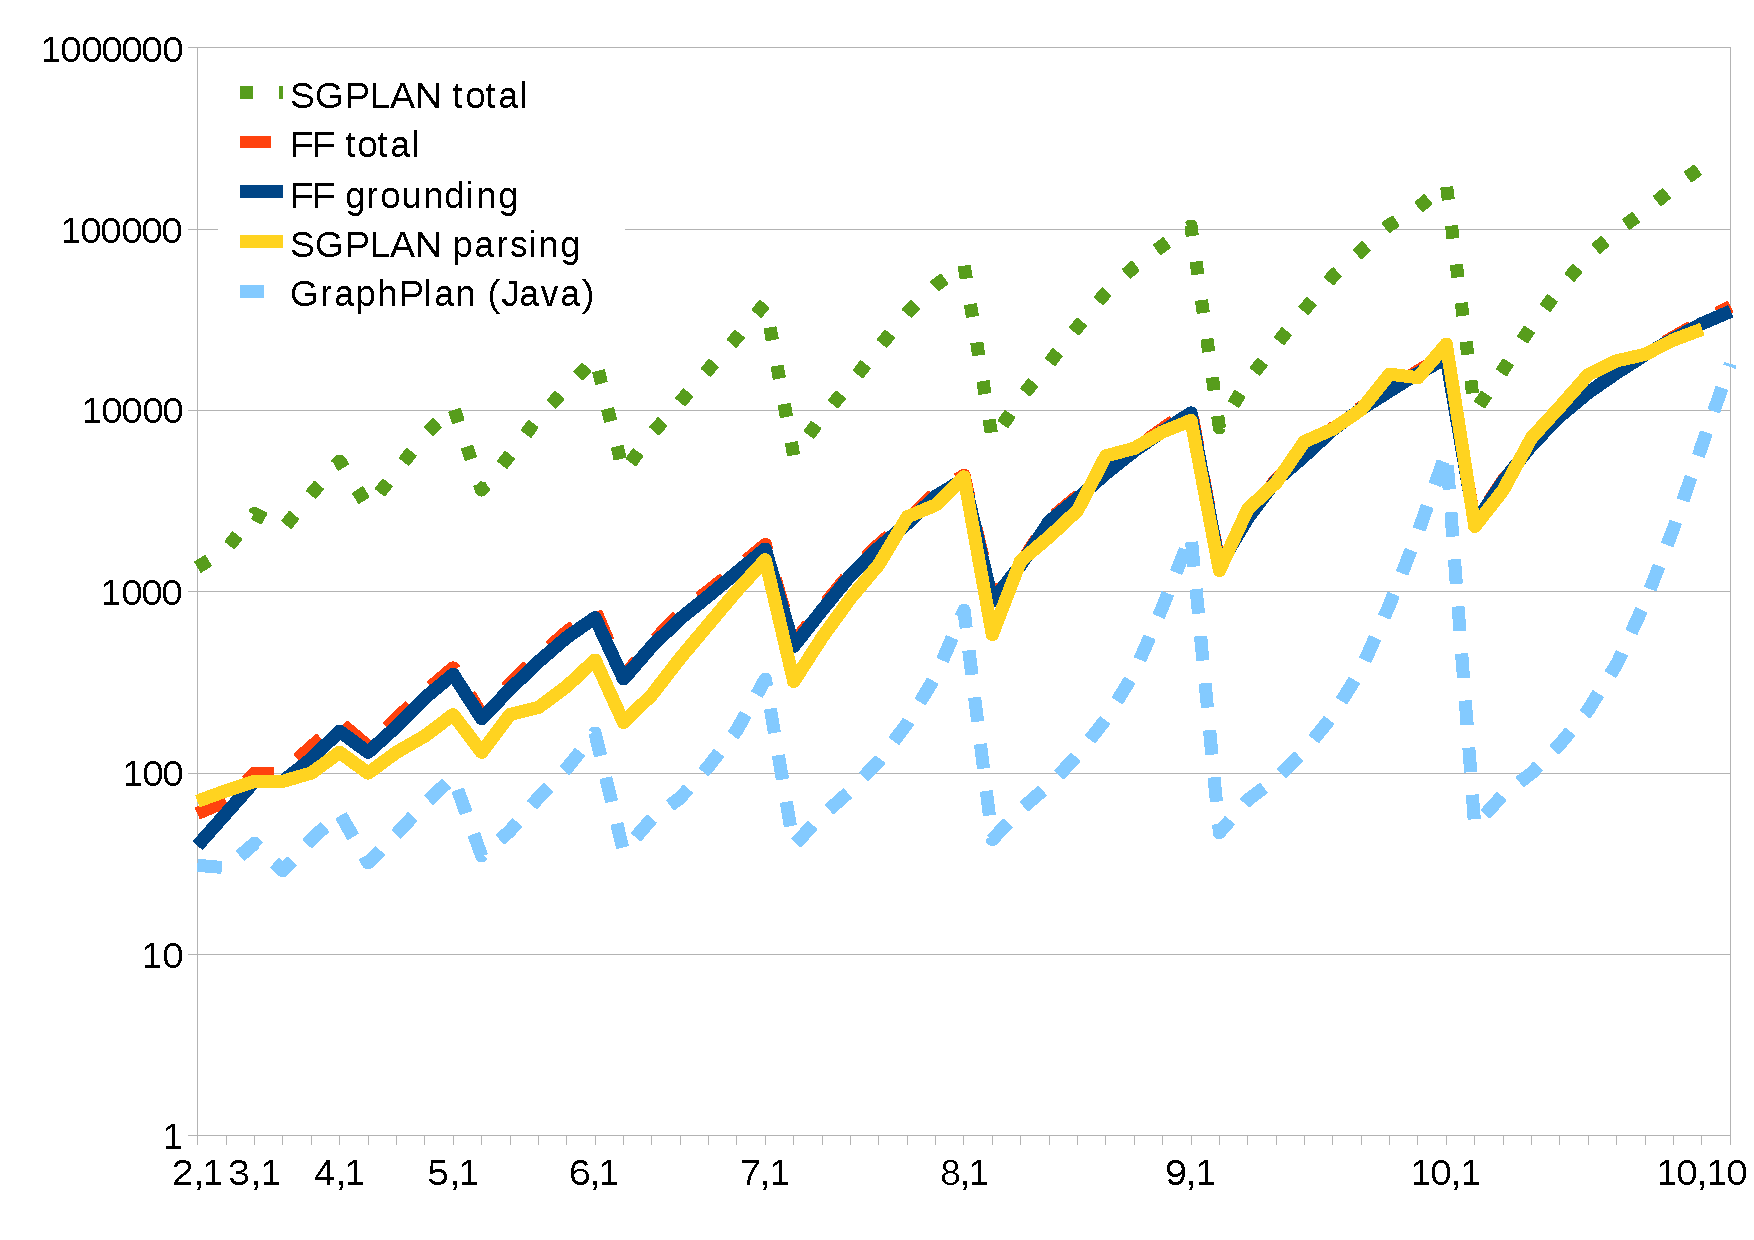
\includegraphics[width=0.75\columnwidth]{graph-exp1}
  %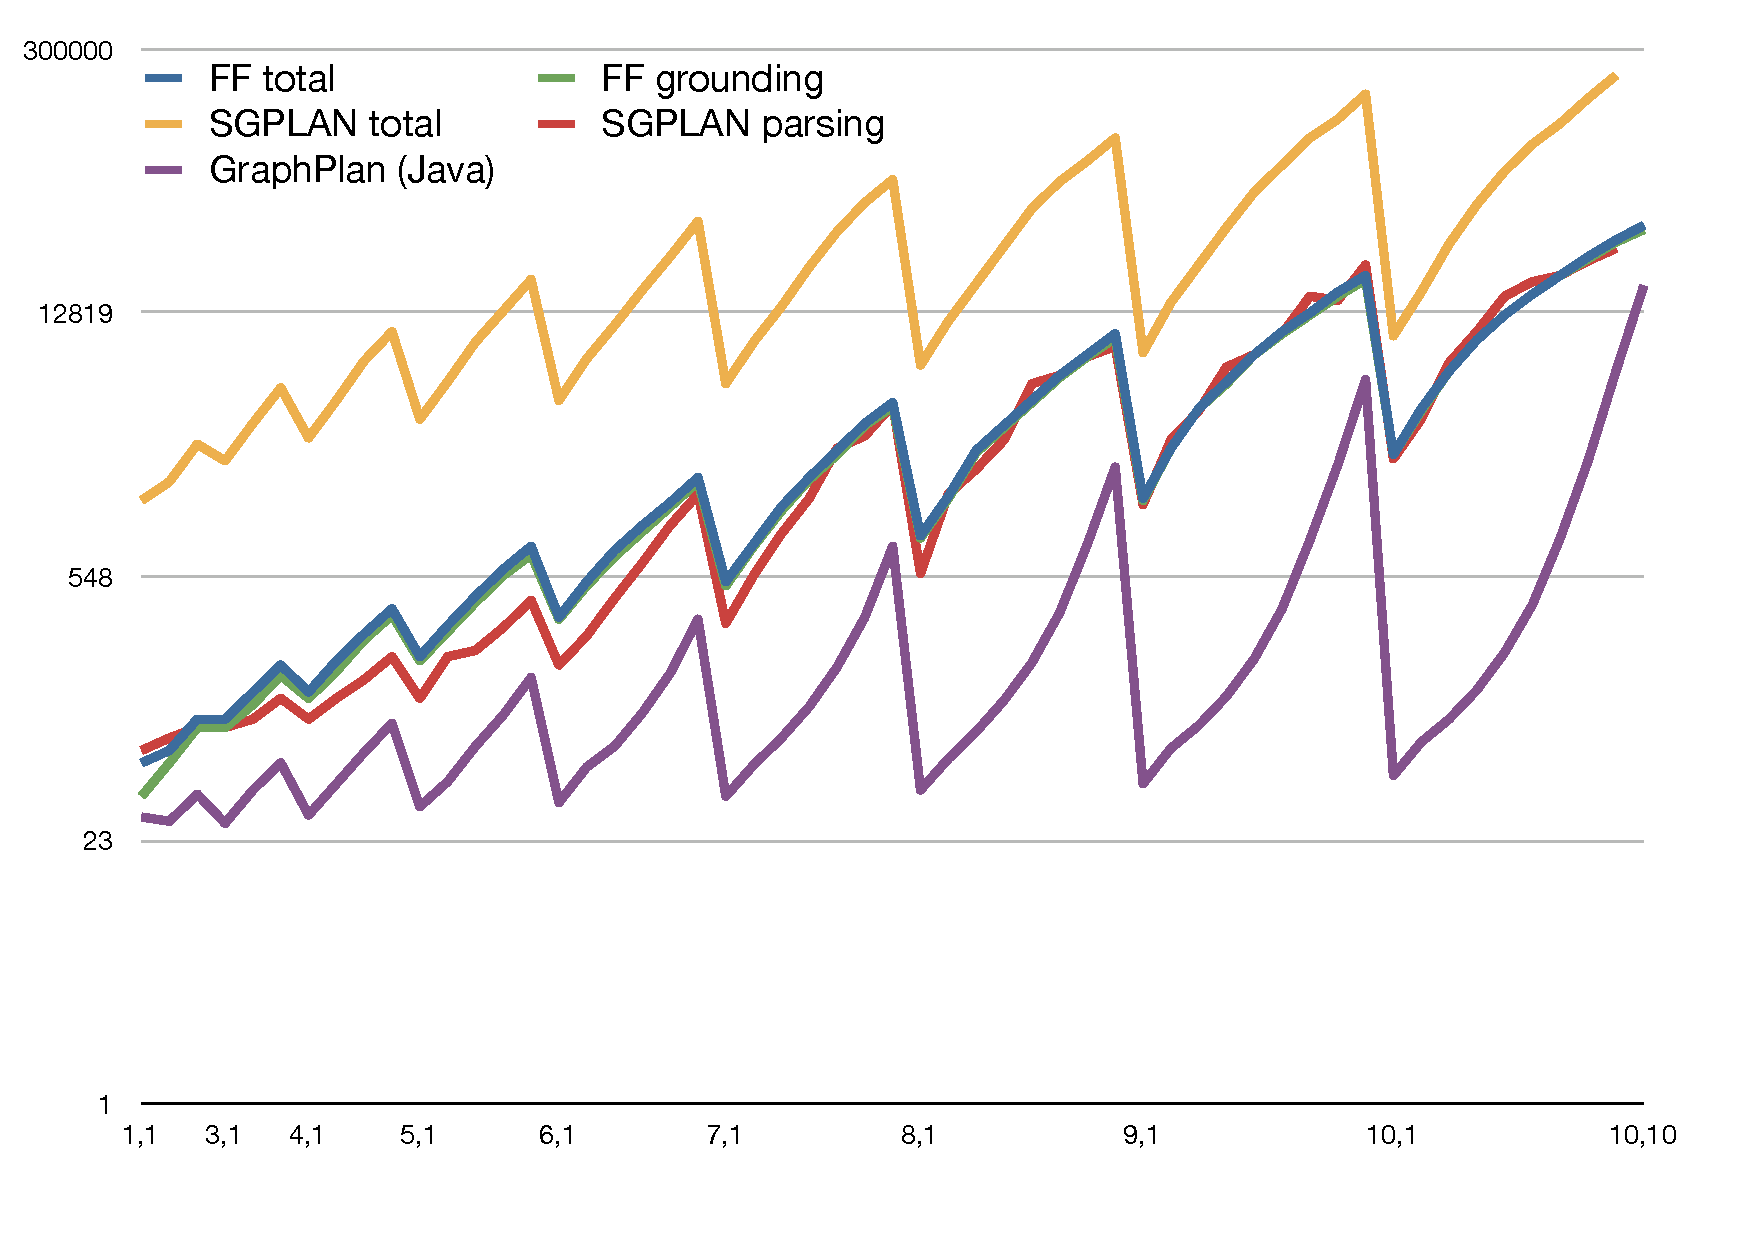
\includegraphics[width=1\columnwidth]{pic-runtime-modifiers-with-sgplan}
  \caption{Results for the sentence generation domain. The
    horizontal axis represents parameters $(m,n)$ from $(1,1)$ to
    $(10,10)$ in lexicographical order. The vertical axis is the
    runtime in milliseconds.}
  \label{fig:runtimes-crisp}
\end{figure}

 The
planners we will use include FF \citep{HoffmannNebel01} and SGPLAN
5.2.2 \citep{hsu06:_new_featur_in_sgplan_for}: These were highly
successful in recent International Planning Competitions and support a
fragment of 

and an ad-hoc implementation
of GraphPlan \citep{Blum1997} written in Java---in our NLG domains. The FF
and SGPLAN planners were chosen due to their success in the International
Planning Competitions. Our implementation of GraphPlan is included as a
counterpoint to the other two, more complex, planners. Most notably, our
version of GraphPlan does not perform a preprocessing ``grounding'' step
like FF and SGPLAN but is much more selective in its predicate and action
instantiations.

The results of this experiment are shown in the graph in
Figure~\ref{fig:runtimes-crisp}. The input parameters $(m,n)$ are plotted
in lexicographic order on the horizontal axis and the runtime is shown in
milliseconds on the vertical axis. These results reveal a number of
interesting insights. First, FF significantly outperforms SGPLAN in this
domain, sometimes by a factor of 10 or more.\footnote{Experiments with
 SGPLAN use a pre-release version of SGPLAN, kindly provided to us by
 Chih-Wei Hsu.The release version of SGPLAN 5.2.2 had a bug which caused it
 to crash on some of our problem instances.}
Second, FF's runtime is dominated by its initial grounding step, in which
it computes the ground instances of all predicates and actions used in the
planning problem in order to avoid unnecessary instantiation during search.
In particular, the ratio of grounding time to total runtime is generally
above 85\%, and rises to above 99\% at $m=11$, which is still a relatively
small universe for this application.\footnote{The
  ``grounding'' time reported here is what FF reports as ``time spent:
  instantiating action templates''.} 

In our testing examples, the time spent by FF on grounding is such that it
is consistently outperformed by our Java implementation of GraphPlan, which
only computes instances of predicates and actions as they are discovered
during the construction of the planning graph. Although FF is consistently
much faster as far as pure search time is concerned, our results indicate
that FF's performance is much more sensitive to the domain size: if we fix
$n=1$, FF takes 60 ms to compute a plan at $m=1$, but 2.4 seconds to
compute the same plan at $m=10$. By comparison, our GraphPlan
implementation takes 30 ms at $m=1$ and still only requires 50 ms at
$m=10$. Conversely, GraphPlan's runtime grows much faster with the plan
size (i.e., with growing values of $n$ for a fixed $m$). Larger, but still
realistically-sized, instances of the sentence generation problem are still
problematic for all the planners we tested.

\subsection{Experiment 2: Sentence generation (XTAG)}
\label{sec:exper-2:-sent-xtag}




\subsection{Experiment 2: Minimal GIVE worlds}
\label{sec:exper-2:-minim}

In the second experiment, we evaluate the performance of the planners on
problems arising in the GIVE domain. We construct a series of test worlds,
similar to the one illustrated in Figure~\ref{fig:give-minimal}. These
worlds consist of a $2n$ by $h$ grid of positions, such that there are
buttons at positions $(2i-1,1)$ and $(2i,h)$ for $1 \leq i \leq n$. The
player starts in position $(1,1)$ and must press all the buttons
to successfully complete the game. The world is generated as a GIVE world
description, and then automatically converted into a planning problem by
the GIVE software. For instance, Figure~\ref{fig:give-planning} shows some
of the actions available in the GIVE domain in PDDL syntax.

\begin{figure}[t]
  \centering
  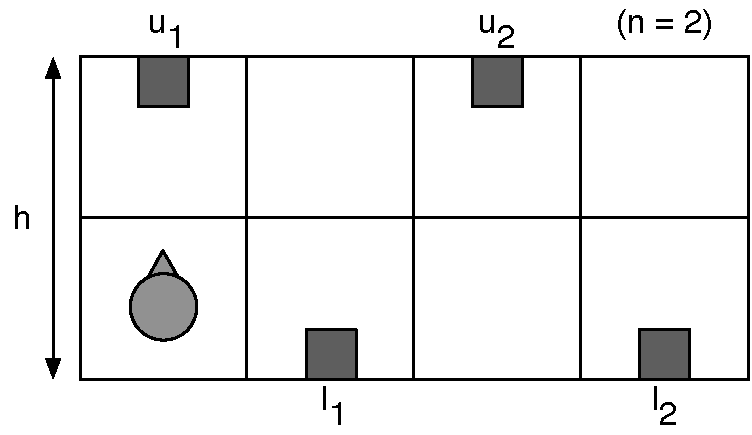
\includegraphics[width=0.5\columnwidth]{pic-buttons}
  \caption{Minimal GIVE world.}
  \label{fig:give-minimal}
\end{figure}

Results for the $h=20$ case, with $n$ ranging from $1$ to $40$, are shown
in Figure~\ref{fig:give-runtime-minimal}. The most obvious result is that
FF is unable to solve any problems beyond $n=13$ on our experimentation
machine within the memory limit of 1 GB. SGPLAN, on the other hand, solves
instances beyond $n=40$ without major problems. In this case, our
implementation of GraphPlan is unable to find any of these plans. The time
spent on grounding is not a major factor in either planner, probably
because the planners need more time to actually compute the plan---for
instance, the optimal plan for the problem $n=40$ has a length of about
1600 steps. As a concrete example, the following is a minimal plan for the
case of a $2$ by $2$ grid with $2$ buttons for the player to press (i.e.,
$n=1$, $h=2$):

\begin{enumerate}
\item $\mathsf{move}(\mathsf{pos\_1\_1},\mathsf{pos\_1\_2}, \mathsf{north})$,
\item $\mathsf{manipulate}\textsf{-}\mathsf{u1}\textsf{-}\mathsf{off}\textsf{-}\mathsf{on}(\mathsf{pos\_1\_2})$,
\item $\mathsf{turn}\textsf{-}\mathsf{right}(\mathsf{north}, \mathsf{east})$,
\item $\mathsf{move}(\mathsf{pos\_1\_2}, \mathsf{pos\_2\_2},
  \mathsf{east})$,
\item $\mathsf{turn}\textsf{-}\mathsf{right}(\mathsf{east}, \mathsf{south})$,
\item $\mathsf{move}(\mathsf{pos\_2\_2}, \mathsf{pos\_2\_1}, \mathsf{south})$,
\item $\mathsf{manipulate}\textsf{-}\mathsf{l1}\textsf{-}\mathsf{off}\textsf{-}\mathsf{on}(\mathsf{pos\_2\_1})$.
\end{enumerate}


\begin{figure}[t]
  \centering
  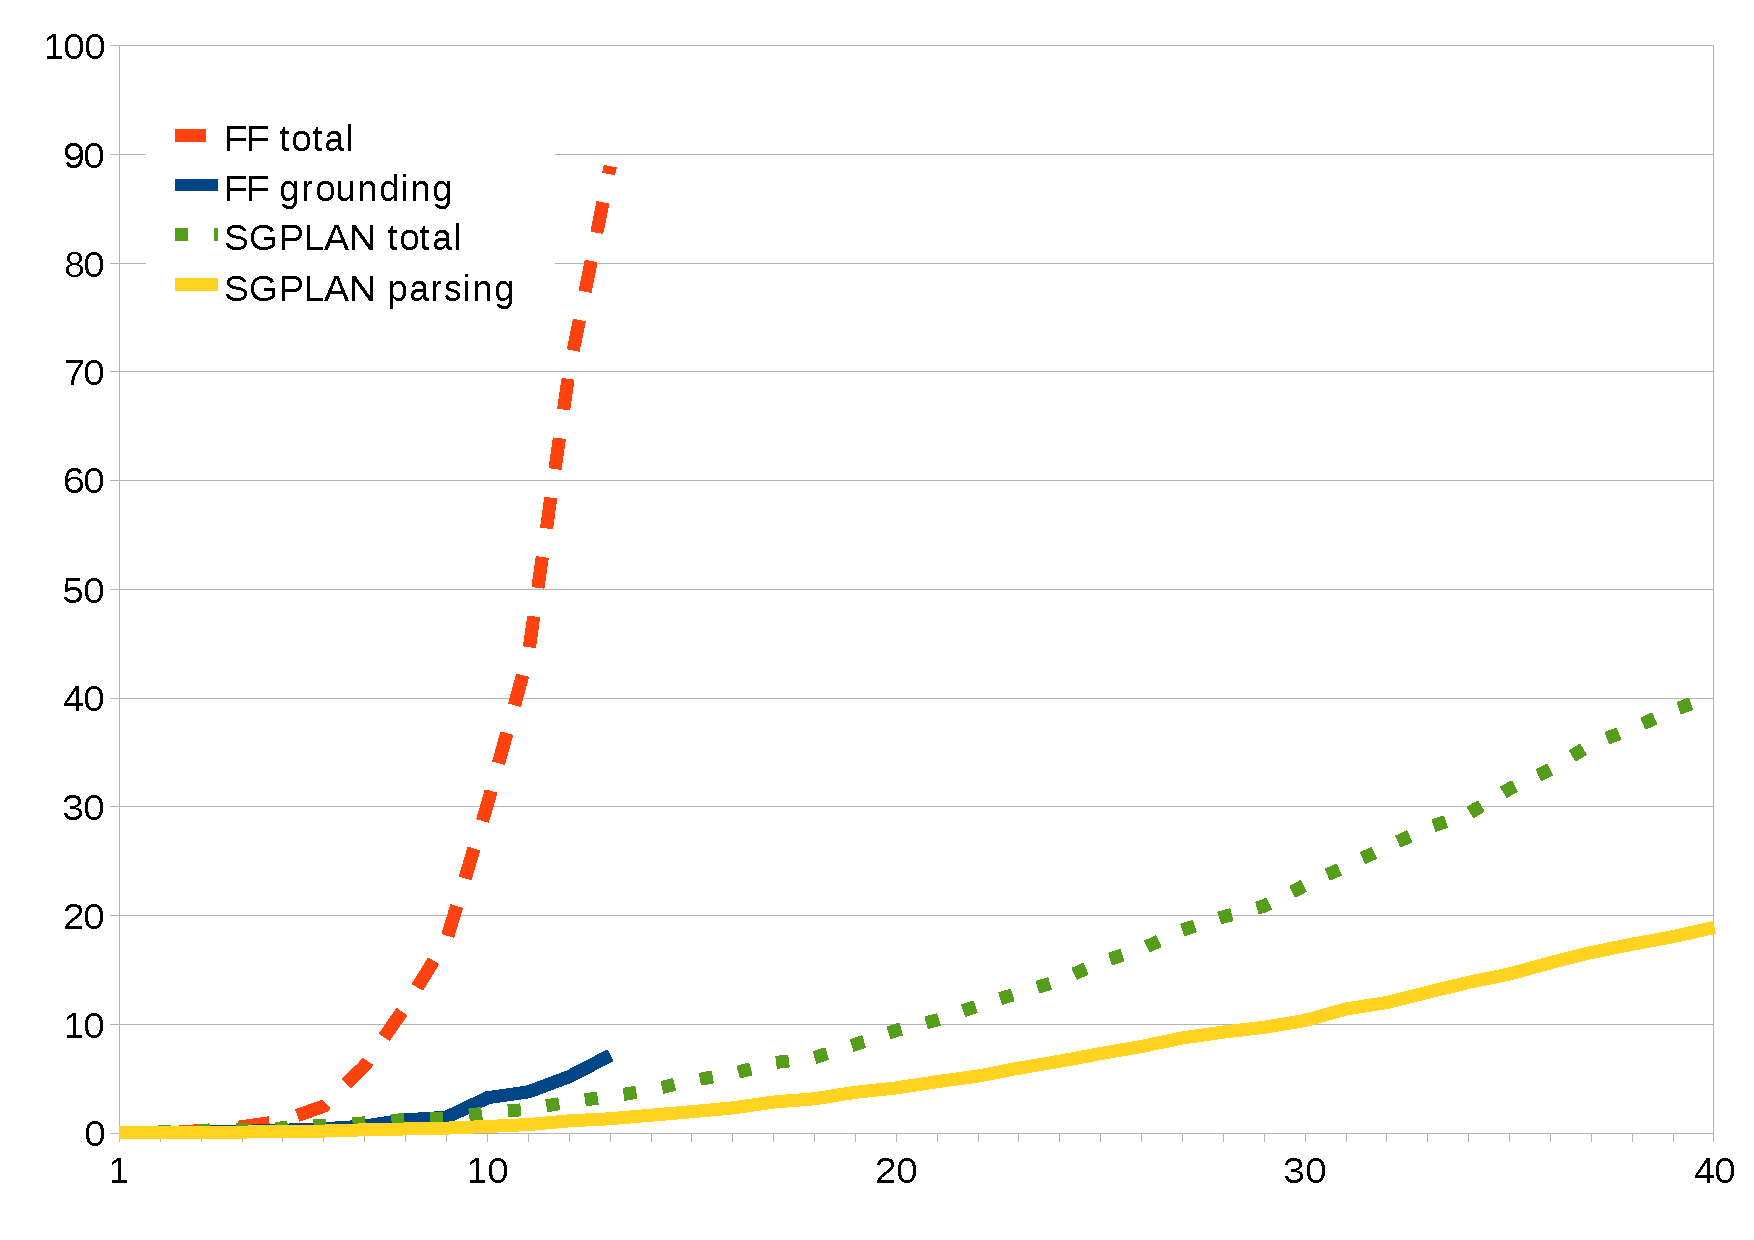
\includegraphics[width=0.75\columnwidth]{graph-exp2}
  %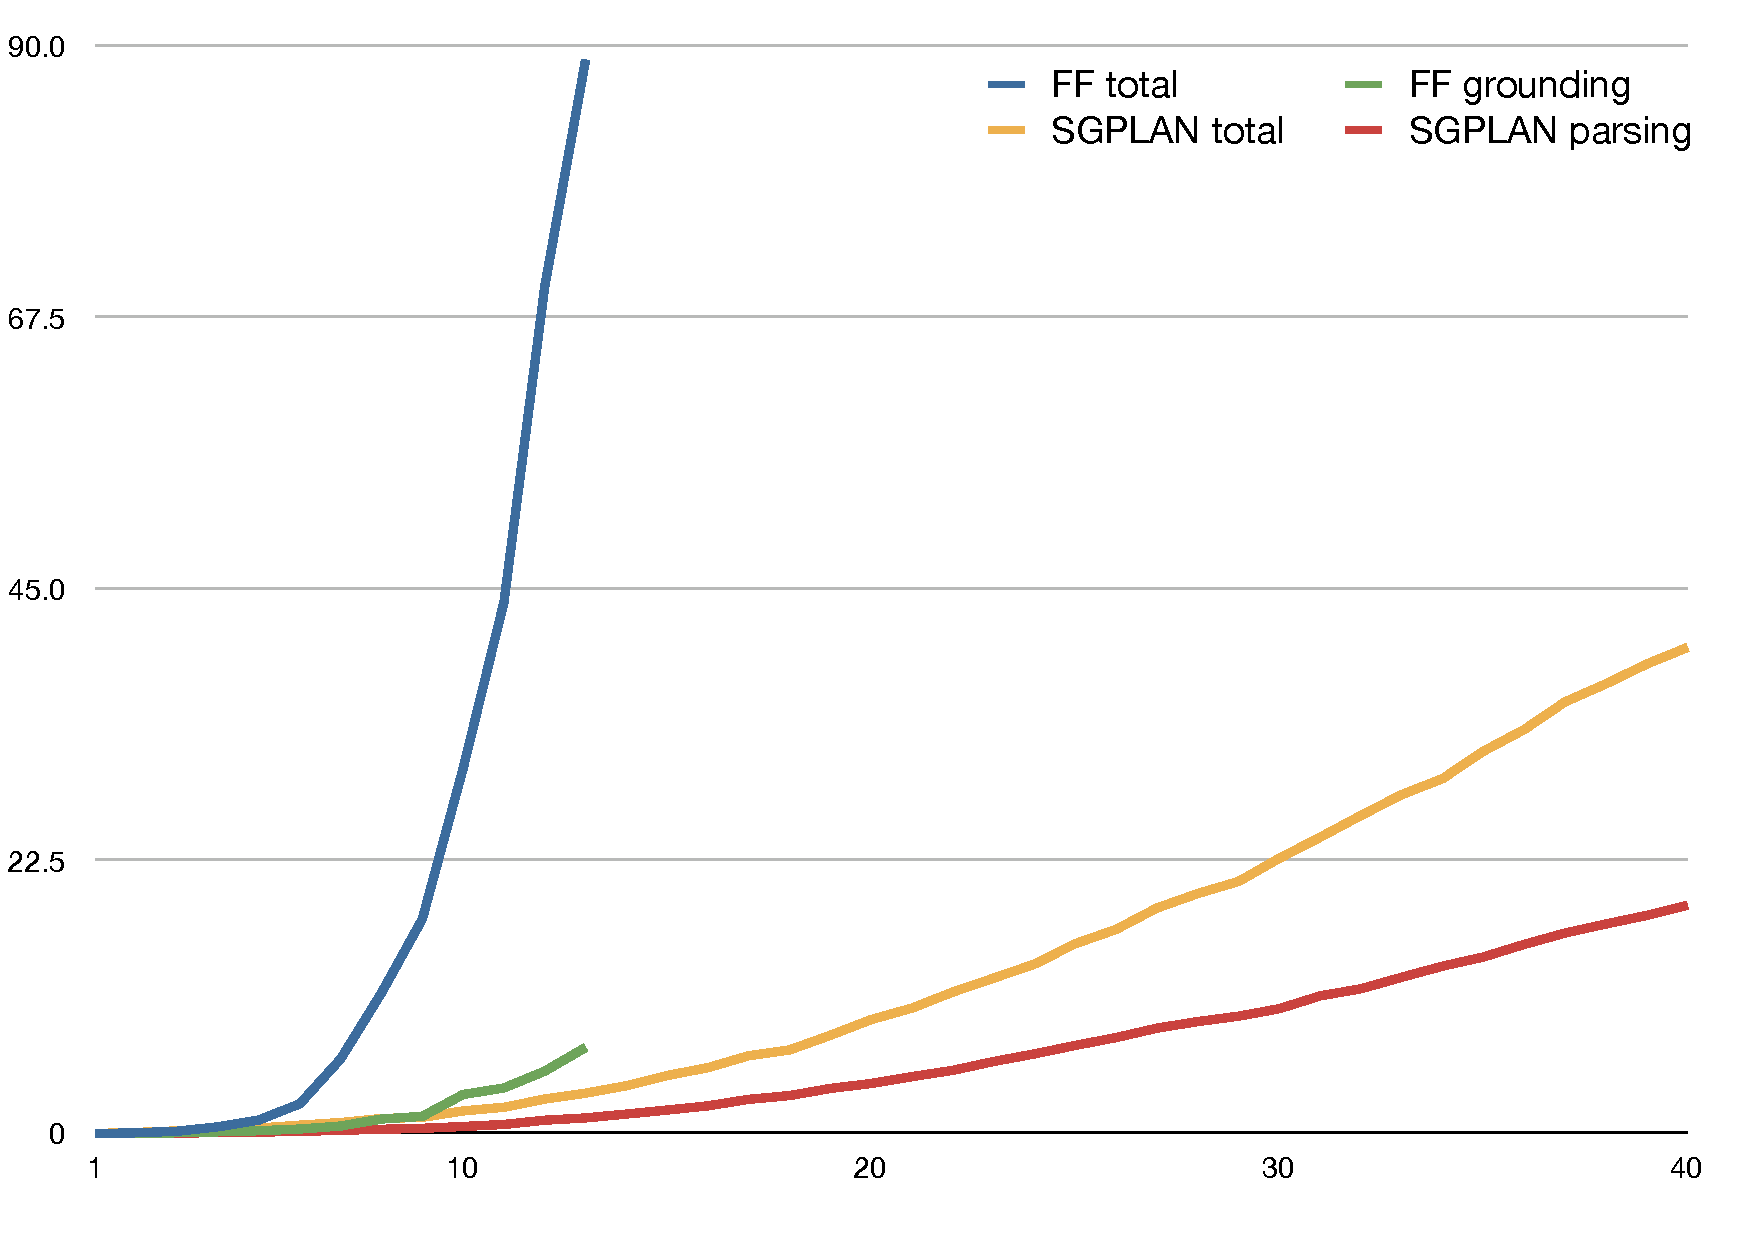
\includegraphics[width=1\columnwidth]{pic-runtime-buttons}
  \caption{Results on the minimal GIVE
    domain for $h=20$. The horizontal axis is $n$. The vertical axis
    is the runtime in seconds.}
  \label{fig:give-runtime-minimal}
\end{figure}


\subsection{Experiment 3: GIVE worlds with extra positions}
\label{sec:experiment-3:-give}

In the third experiment, we vary the structure of the GIVE world in order
to judge the effect that universe size has on the planning problem in this
domain. Starting with the ordinary GIVE world described in Experiment~2, we
extend the world map by adding another $w$ by $h$ empty ``junk'' positions
to the right of the minimal world, as shown in Figure~\ref{fig:give-junk}.
These new positions are not actually required in any plan, but extend the
size of the state space and approximate the situation in the actual GIVE
domain where most grid positions are never used. We leave the initial state
and goal untouched. As before, we generate a GIVE world description and
then convert it into a planning problem in PDDL.

\begin{figure}[t]
  \centering
  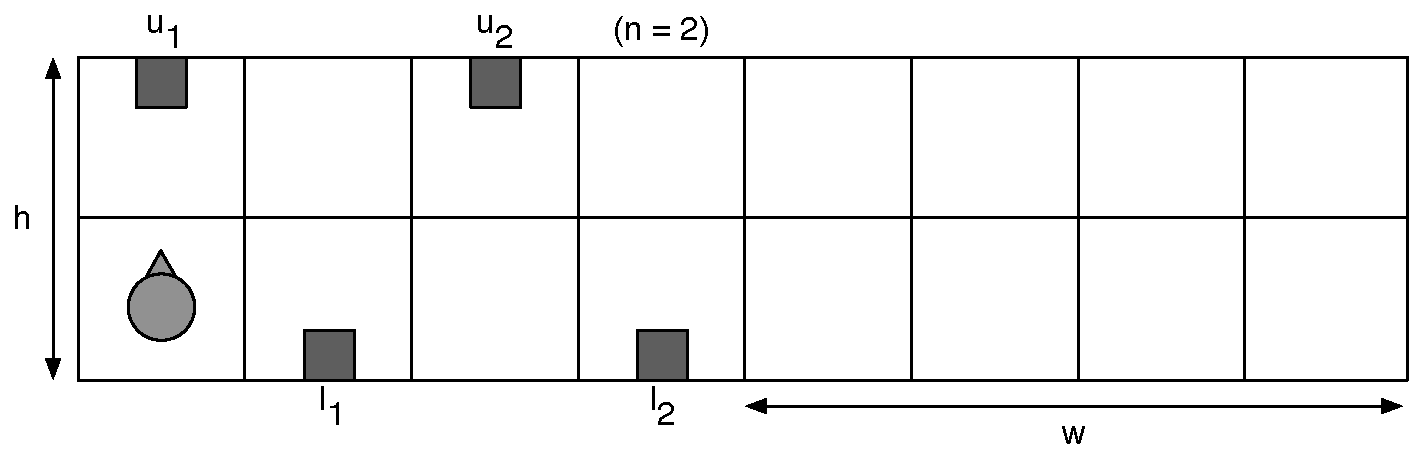
\includegraphics[width=0.80\columnwidth]{pic-empty-buttons}
  \caption{GIVE world with extra ``junk'' positions.}
  \label{fig:give-junk}
\end{figure}

Results for the $h=20$, $n=5$ case with $w$ ranging from $1$ to $70$ are
shown in Figure~\ref{fig:give-runtime-junk}. As in Experiment~2, FF again
runs out of memory, this time at $w=17$, while SGPLAN easily solves inputs
beyond $w=70$. As in Experiment~2, our implementation of GraphPlan is
unable to generate any of these plans. Unlike Experiment 2, however, both
FF and SGPLAN now spend a substantial proportion of their time on
grounding. In SGPLAN, this translates to a ``parsing time'' (which we
assume includes grounding) which grows from 180 ms to 21.7 seconds as $w$
grows from $1$ to $75$. The rest of the runtime, which also includes the
search time, only grows from 400 ms to 2.3 seconds. This difference is
particularly dramatic given that the actual optimal plan in each case is an
identical plan of about 100 steps (i.e., the one we would have found in
Experiment 2 for the $h=20$, $n=5$ case). The planning times for these
instances are also concerning since times over a couple seconds will
negatively affect the overall response time of the system, which must react
in real time to user actions.

\begin{figure}[t]
  \centering
  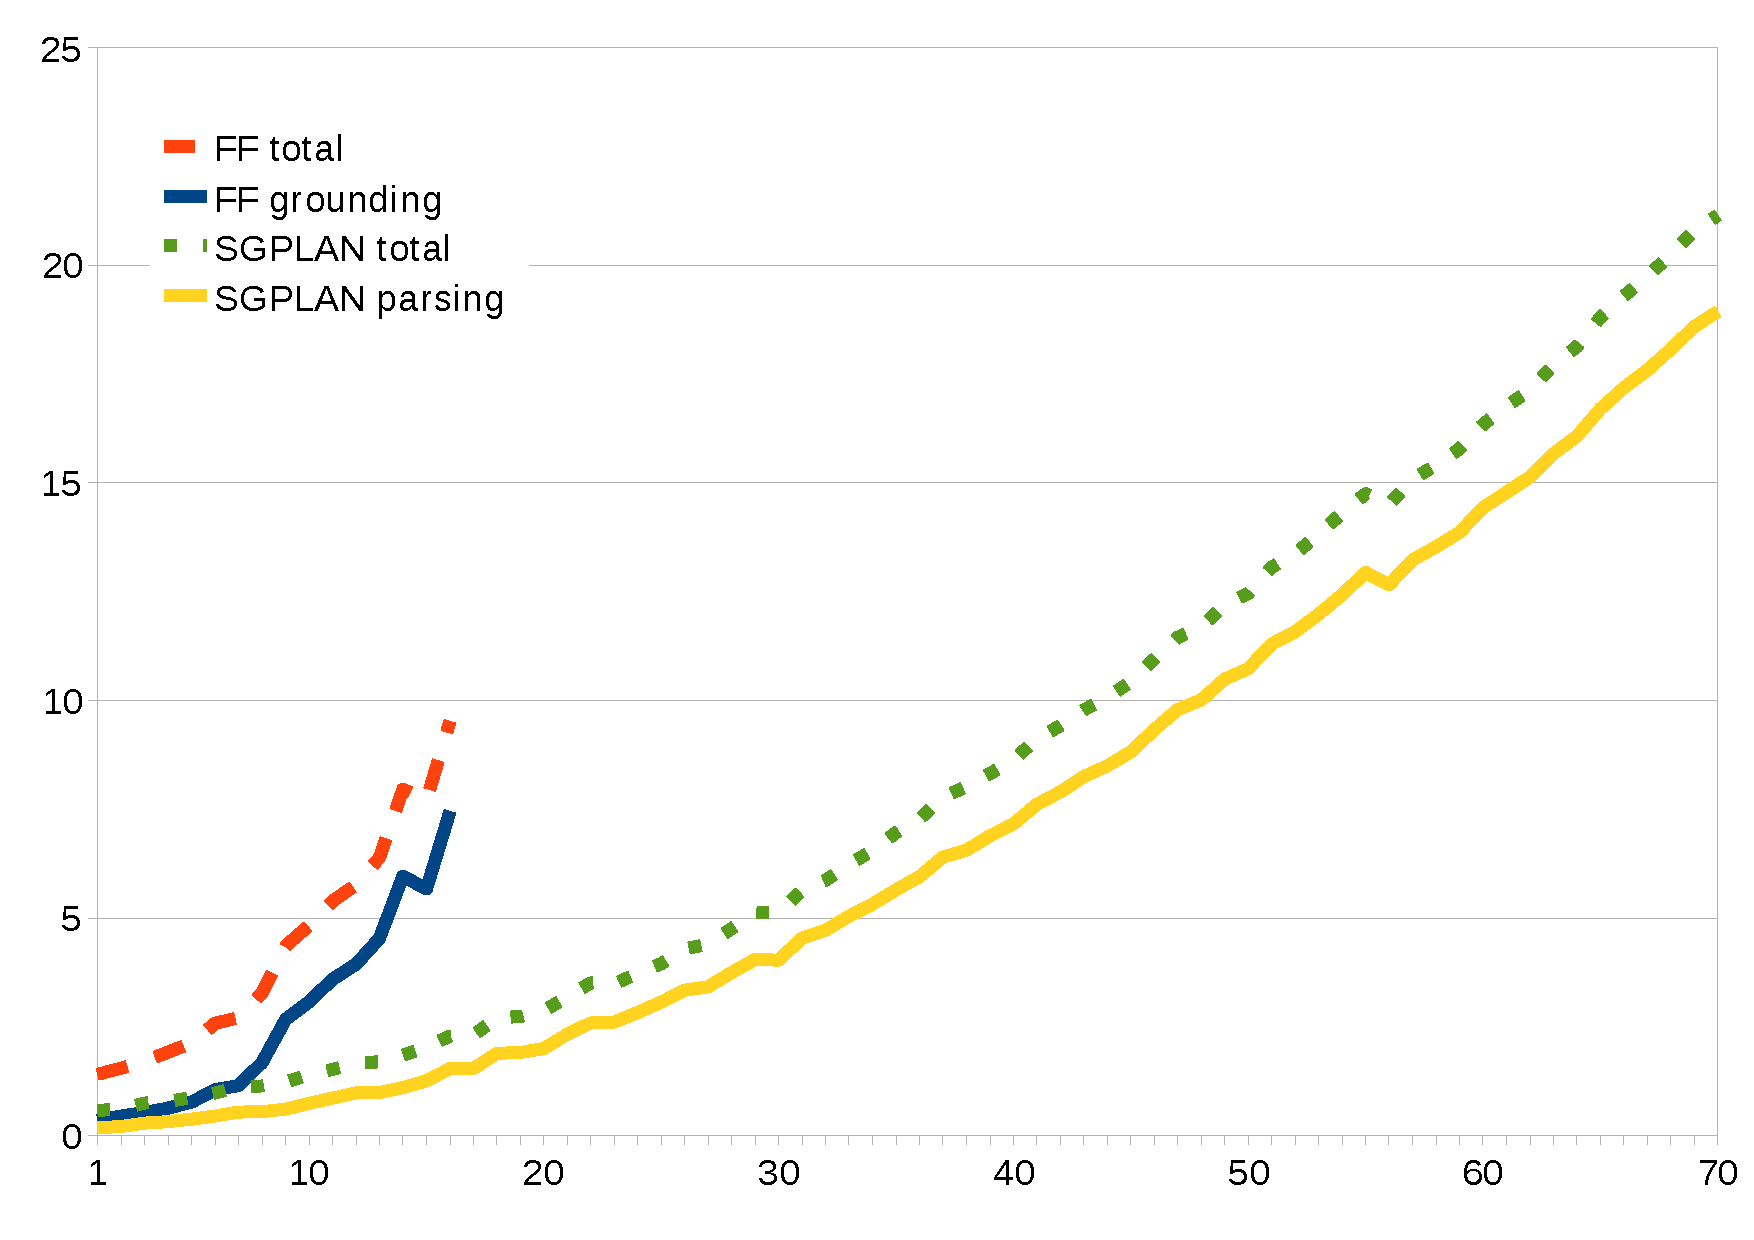
\includegraphics[width=0.75\columnwidth]{graph-exp3}
  %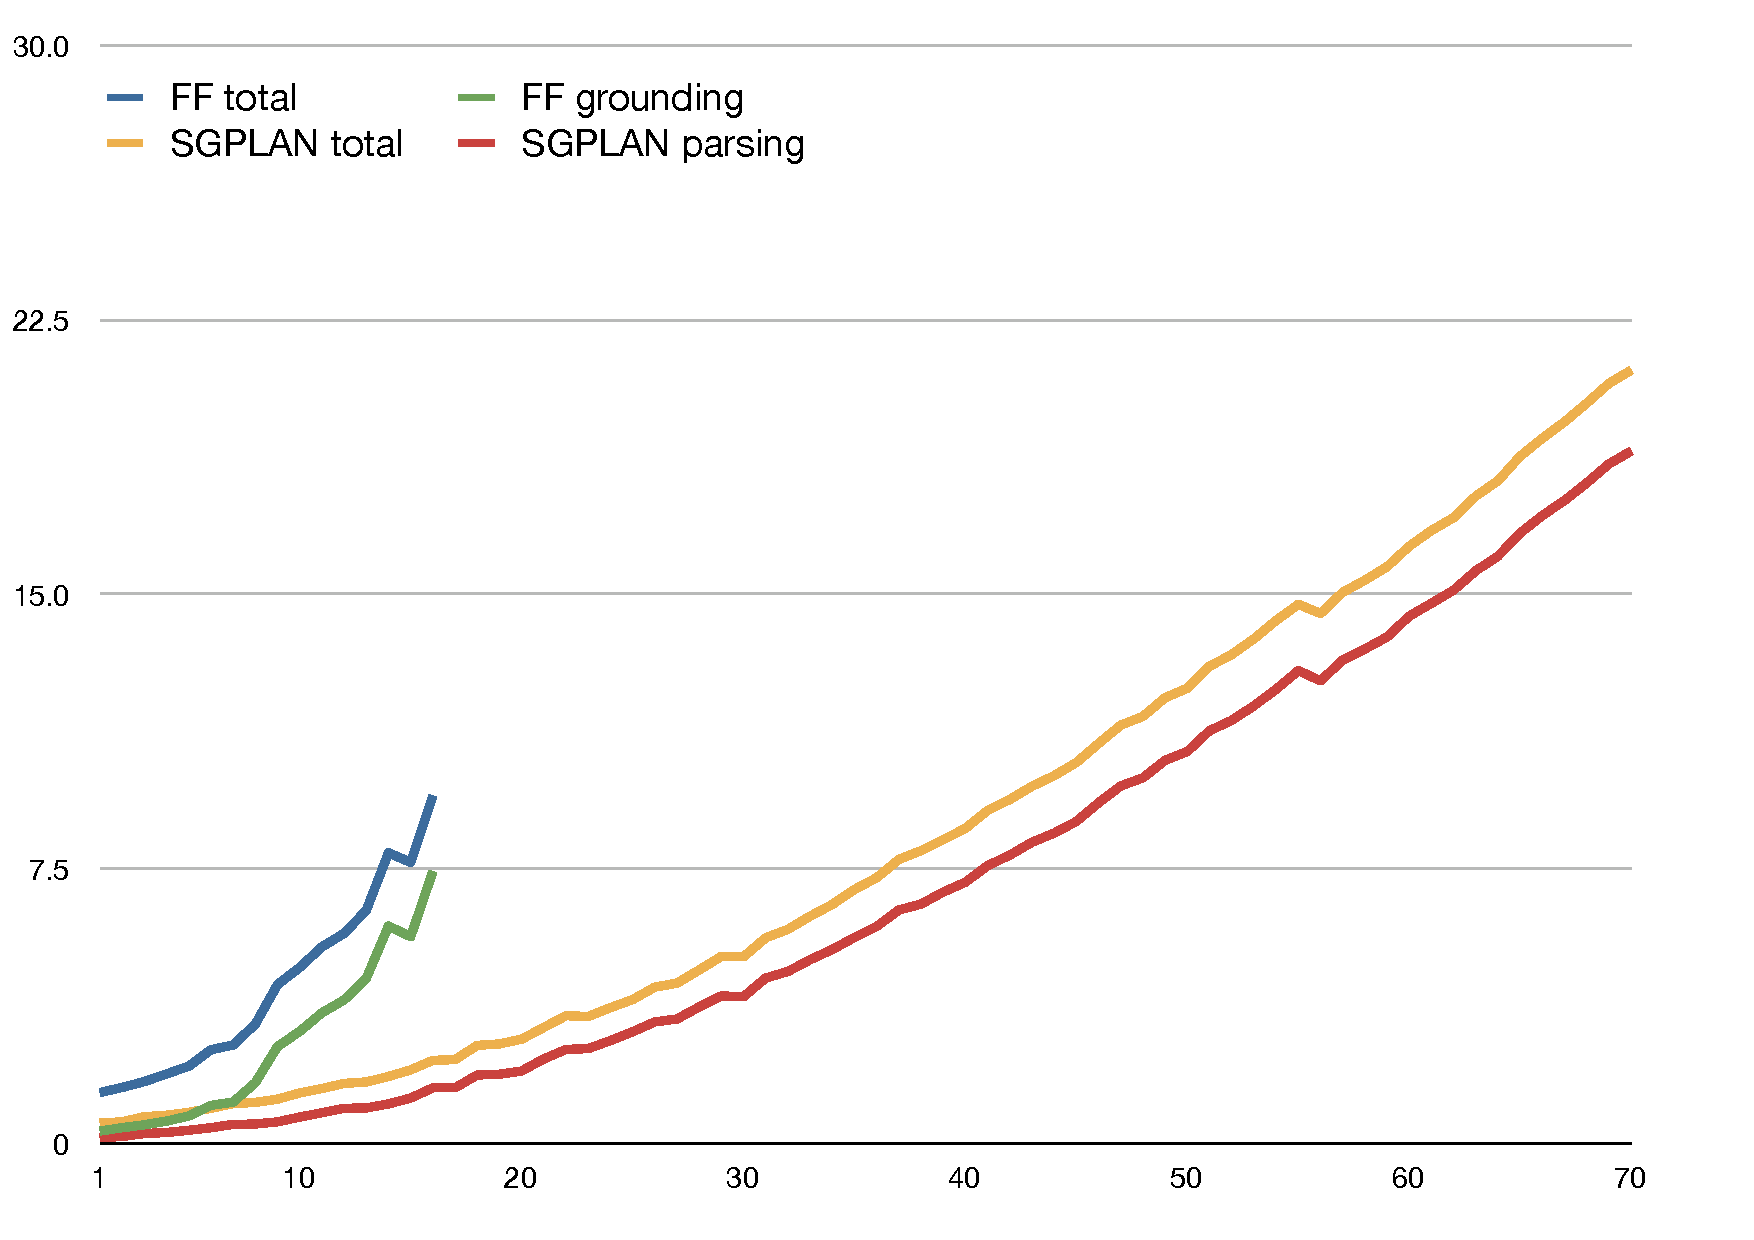
\includegraphics[width=1\columnwidth]{pic-runtime-empty-world}
  \caption{Results on the GIVE domain with junk
    positions for $h=20$ and $n=5$. The horizontal axis is $w$.
    The vertical axis is the runtime in seconds.}
  \label{fig:give-runtime-junk}
\end{figure}


\subsection{Experiment 4: GIVE worlds with inaccessible positions}
\label{sec:experiment-4:-give}

In the final experiment, we consider a variation on the GIVE worlds from
Experiment~3. As before, we begin with a base grid of $2n$ by $h$
positions, with buttons at positions $(2i-1,1)$ and $(2i,h)$ for $1 \leq i
\leq n$. We then generate a second grid of $w$ by $h$ positions and place
an additional button in this grid. Unlike Experiment~3, the second grid
does not extend the first grid but is ``disconnected'' so its positions are
inaccessible from the first grid, as shown in
Figure~\ref{fig:give-junk-nosoln}. Since the geometry of the grid makes it
impossible to construct a plan for pressing all the buttons in the world,
we instead investigate the time it takes a planner to arrive at the
conclusion that the problem cannot be solved.

Results for the $h=20$, $n=5$ case with $w$ ranging from 1 to 50 are shown
in Figure~\ref{fig:give-runtime-nosoln}.\footnote{FF and SGPLAN do
 not display runtimes when they fail to construct a plan so an external timing
 program was used to generate these results.}
In this case, the runtimes for FF rise sharply around $w=28$, producing
times that are unacceptable for an NLG system in practice. FF is unable
to complete problem instances above $w=35$. SGPLAN, by comparison, performs
exceptionally well and is able to complete problems instances up to $w=50$
in about 0.3 seconds and $w=80$ in about 0.6 seconds. These results
demonstrate that SGPLAN has a significant advantage over FF in this
experiment. 
%Our implementation of GraphPlan is unable to complete any of
%these problem instances.

\begin{figure}[t]
  \centering
  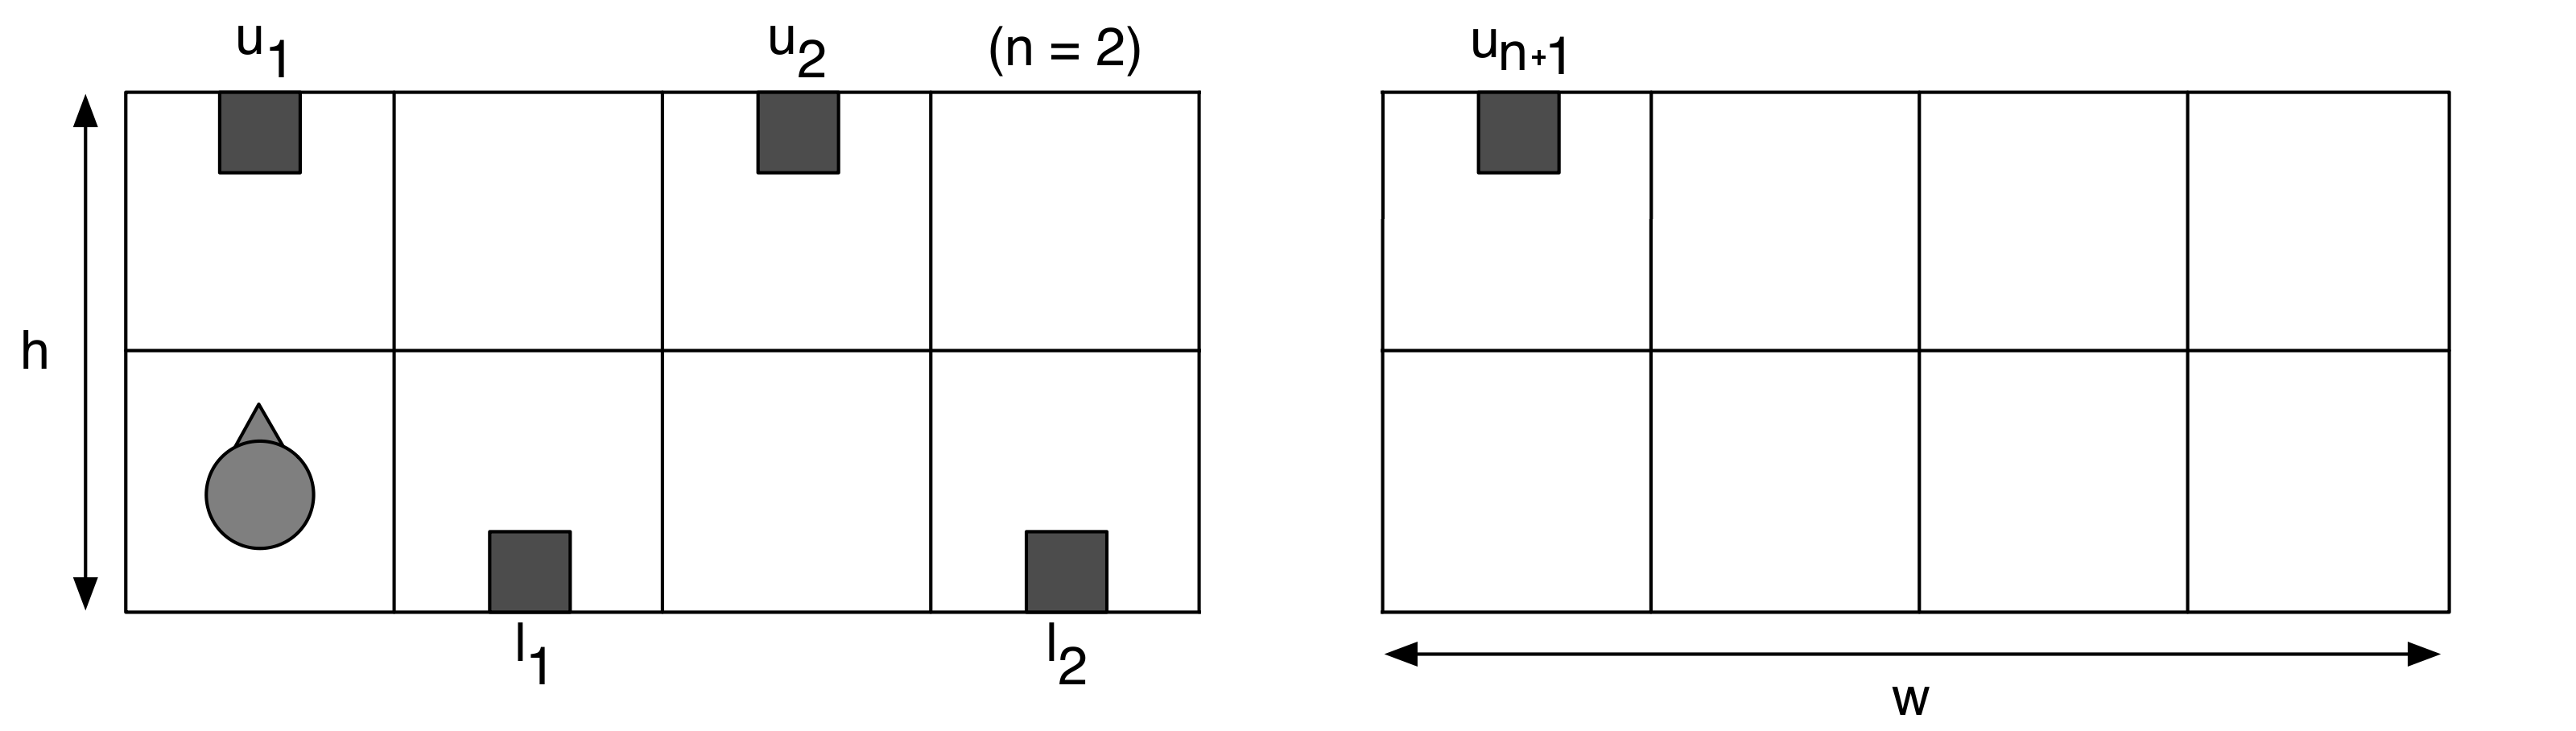
\includegraphics[width=0.85\columnwidth]{pic-empty-inaccessible}
  \caption{GIVE world with inaccessible positions.}
  \label{fig:give-junk-nosoln}
\end{figure}

\begin{figure}
  \centering
  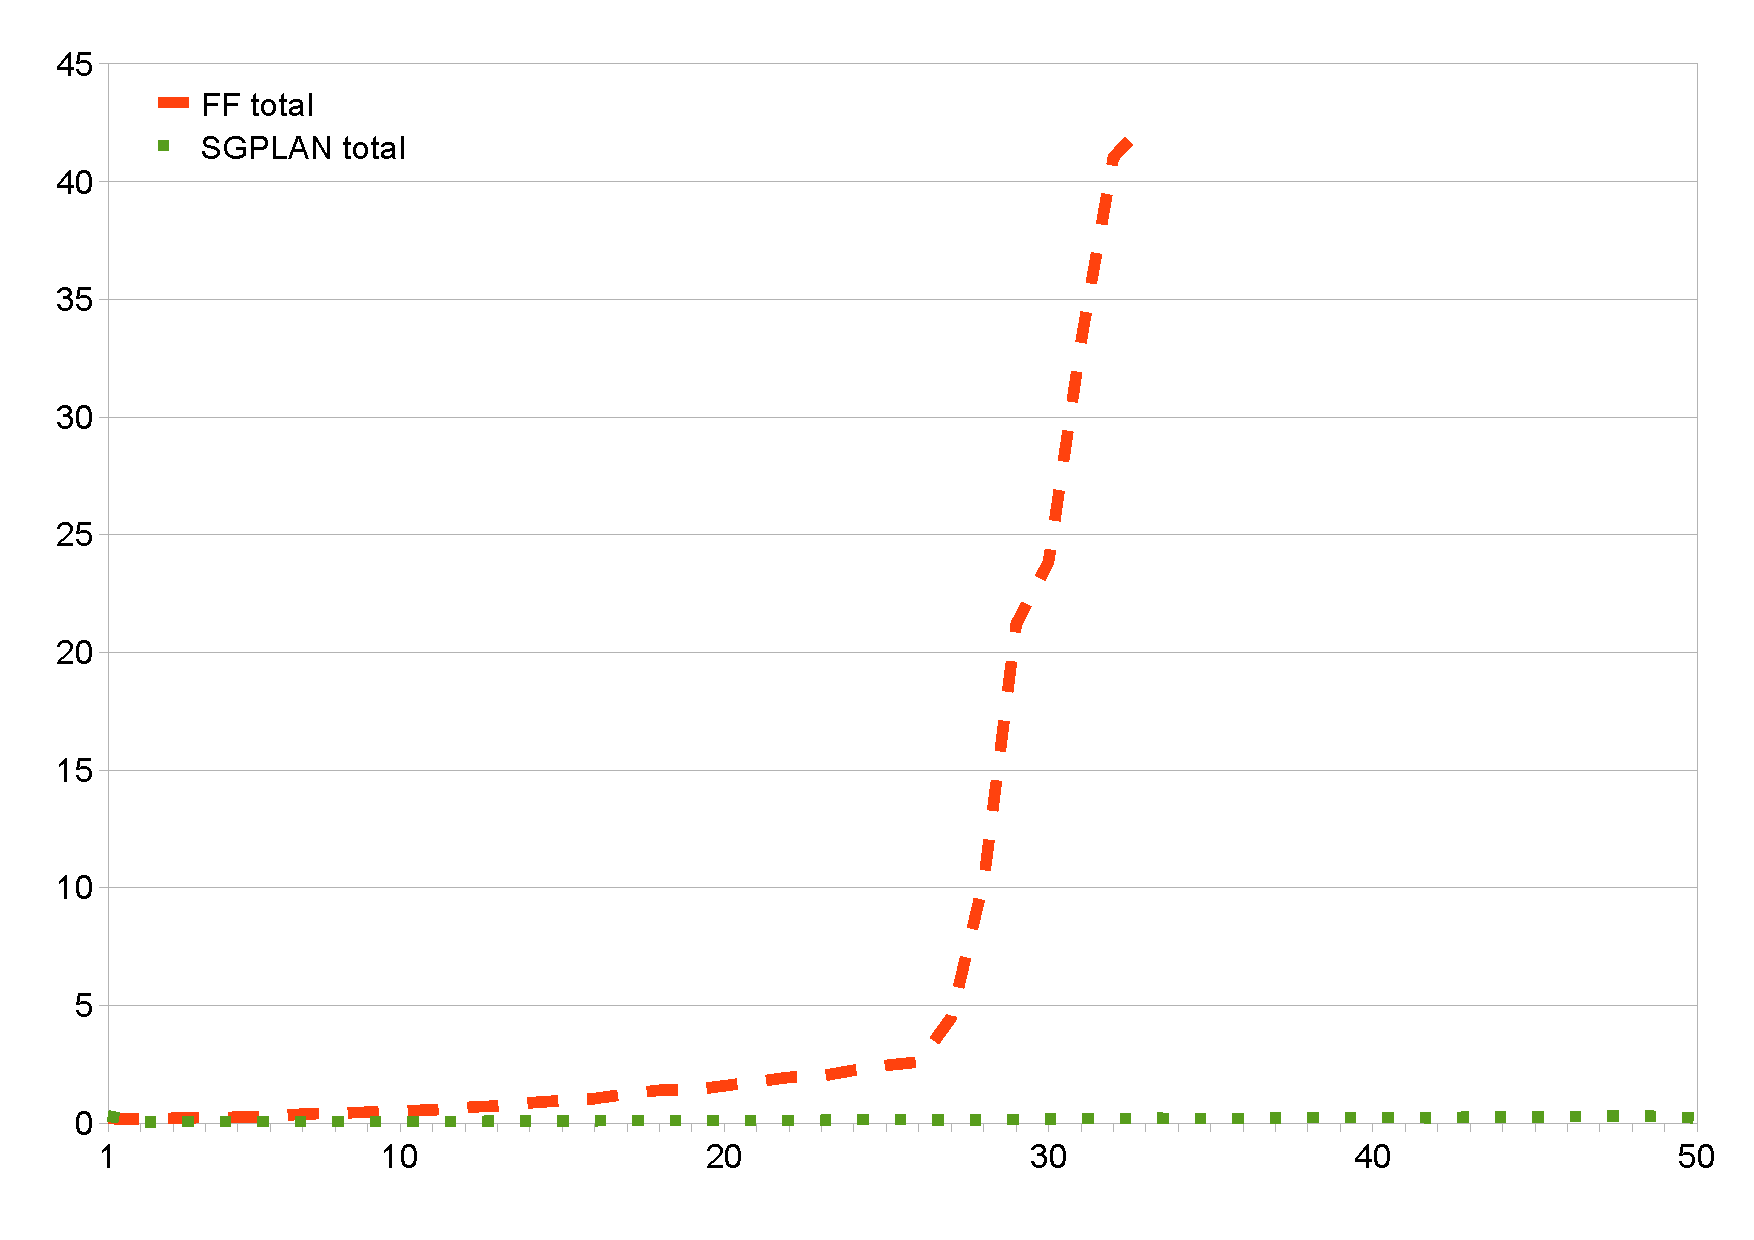
\includegraphics[width=0.85\columnwidth]{graph-exp4}
  %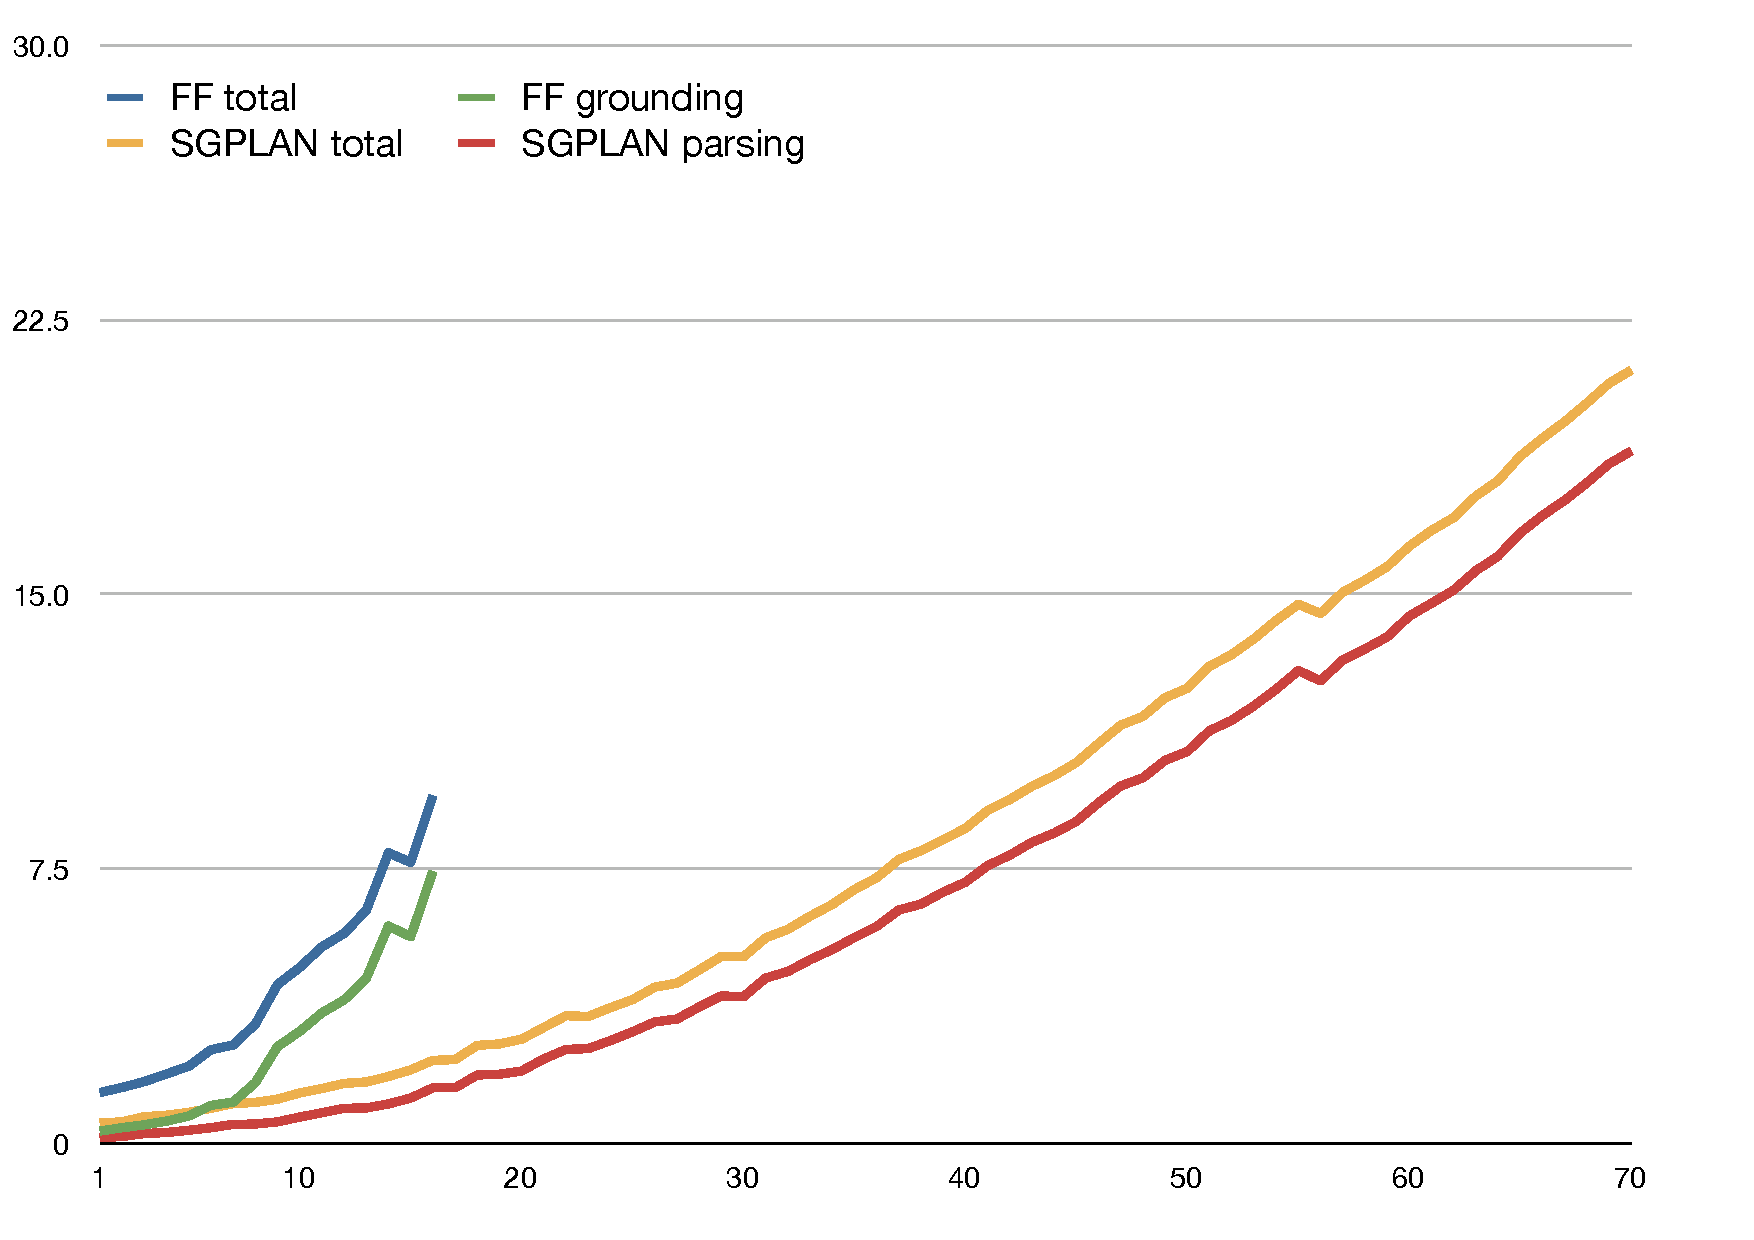
\includegraphics[width=1\columnwidth]{pic-runtime-empty-world}
  \caption{Results on the GIVE domain with inaccessible
    positions for $h=20$ and $n=5$. The horizontal axis is $w$.
    The vertical axis is the runtime in seconds.}
  \label{fig:give-runtime-nosoln}
\end{figure}



%%% Local Variables: 
%%% mode: latex
%%% TeX-master: "manuscript"
%%% End: 
